%!TEX TS-program = xelatex
\documentclass[10pt, compress]{beamer}

\usetheme[usetitleprogressbar]{m}

\usepackage[export]{adjustbox}
\usepackage{etoolbox}
\usepackage{booktabs}
\usepackage{dcolumn}
\usepackage[scale=2]{ccicons}
\usepackage{color}

% math typesetting
\usepackage{array}
\usepackage{amsmath}
\usepackage{amssymb}
\usepackage{amsthm}
\usepackage{amsfonts}
\usepackage{relsize}
\usepackage{mathtools}
\usepackage{bm}

% tables
\usepackage{tabularx}
\usepackage{booktabs}
\usepackage{multicol}
\usepackage{multirow}

% graphics stuff
\usepackage{subfig}
\usepackage{graphicx}
\usepackage[space]{grffile} % allows us to specify directories that have spaces
\usepackage{tikz}

% to change enumeration symbols begin{enumerate}[(a)]
\usepackage{enumerate}

% Add some colors
\definecolor{red1}{RGB}{253,219,199}
\definecolor{red2}{RGB}{244,165,130}
\definecolor{red3}{RGB}{178,24,43}

\definecolor{green1}{RGB}{229,245,224}
\definecolor{green2}{RGB}{161,217,155}
\definecolor{green3}{RGB}{49,163,84}

\definecolor{blue0}{RGB}{255,247,251}
\definecolor{blue1}{RGB}{222,235,247}
\definecolor{blue2}{RGB}{158,202,225}
\definecolor{blue3}{RGB}{49,130,189}
\definecolor{blue4}{RGB}{4,90,141}

\definecolor{purple1}{RGB}{191,211,230}
\definecolor{purple2}{RGB}{140,150,198}
\definecolor{purple3}{RGB}{140,107,177}

\definecolor{brown1}{RGB}{246,232,195}
\definecolor{brown2}{RGB}{223,194,125}
\definecolor{brown3}{RGB}{191,129,45}

% square bracket matrices
\let\bbordermatrix\bordermatrix
\patchcmd{\bbordermatrix}{8.75}{4.75}{}{}
\patchcmd{\bbordermatrix}{\left(}{\left[}{}{}
\patchcmd{\bbordermatrix}{\right)}{\right]}{}{}

% easy command for boldface math symbols
\newcommand{\mbs}[1]{\boldsymbol{#1}}

% command for R package font
\newcommand{\pkg}[1]{{\fontseries{b}\selectfont #1}}

% approx iid
\newcommand\simiid{\stackrel{\mathclap{\normalfont\mbox{\tiny{iid}}}}{\sim}}

% references to graphics
\makeatletter
\def\input@path{{/Users/janus829/Dropbox/Research/netModels/summResults/}, {/Users/s7m/Dropbox/Research/netModels/summResults/}, {/Users/mdw/Dropbox/Research/netModels/summResults/}}
\graphicspath{{/Users/janus829/Dropbox/Research/netModels/summResults/}, {/Users/s7m/Dropbox/Research/netModels/summResults/},{/Users/mdw/Dropbox/Research/netModels/summResults/}}

\title[AMEN]{\textsc{AMEN for Latent Factor Models}}
\author[Minhas, Hoff, \& Ward]{Shahryar Minhas$^\dag$, Peter D. Hoff$^\ddag$, \& Michael D. Ward$^\dag$ \\ Duke University \\ $^\dag$ Department of Political Science \\ $^\ddag$ Department of Statistical Science} 

\date{\today}

\begin{document}
\frame{\titlepage}

%%%%%%%%%%%%%%%%%%%%%%%%%%%%%%%%%%%%%%%%%%%%%%%%%%%%%%%%%%%%
\frame
{
  \frametitle{Motivation}
  
  Relational data are composed of interactions between actors that are interdependent 

\small{
\begin{table}[ht]
  \captionsetup{justification=raggedright }
  \centering
  \begin{minipage}{.45\textwidth}
    \centering
    \begingroup
    \setlength{\tabcolsep}{10pt}
    \begin{tabular}{ccc}
      Sender & Receiver & Event \\
      \hline\hline
      $i$ & $j$ & $y_{ij}$ \\
      \multirow{2}{*}{\vdots} & $k$ & $y_{ik}$ \\
      ~ & $l$ & $y_{il}$ \\
      $j$ & $i$ & $y_{ji}$ \\
      \multirow{2}{*}{\vdots} & $k$ & $y_{jk}$ \\
      ~ & $l$ & $y_{jl}$ \\
      $k$ & $i$ & $y_{ki}$ \\
      \multirow{2}{*}{\vdots} & $j$ & $y_{kj}$ \\
      ~ & $l$ & $y_{kl}$ \\
      $l$ & $i$ & $y_{li}$ \\
      \multirow{2}{*}{\vdots} & $j$ & $y_{lj}$ \\
      ~ & $k$ & $y_{lk}$ \\
      \hline\hline
    \end{tabular}
    \endgroup
    % \caption{Structure of datasets used in canonical design.} 
    % \label{tab:canDesign}
  \end{minipage}
  $\mathbf{\longrightarrow}$
  \begin{minipage}{.45\textwidth}
    \centering
    \begingroup
    \setlength{\tabcolsep}{10pt}
    \renewcommand{\arraystretch}{1.5}
    \begin{tabular}{c||cccc}
    ~ & $i$ & $j$ & $k$ & $l$ \\ \hline\hline
    $i$ & \footnotesize{NA} & $y_{ij}$ & $y_{ik}$ & $y_{il}$ \\
    $j$ & $y_{ji}$ & \footnotesize{NA}  & $y_{jk}$ & $y_{jl}$ \\
    $k$ & $y_{ki}$ & $y_{kj}$ & \footnotesize{NA}  & $y_{kl}$ \\
    $l$ & $y_{li}$ & $y_{lj}$ & $y_{lk}$ & \footnotesize{NA}  \\
    \end{tabular}
    \endgroup
    % \caption{Adjacency matrix representation of data in Table~\ref{tab:canDesign}. Senders are represented by the rows and receivers by the columns. }
    % \label{tab:netDesign}
  \end{minipage}
\end{table}
}

} 
%%%%%%%%%%%%%%%%%%%%%%%%%%%%%%%%%%%%%%%%%%%%%%%%%%%%%%%%%%%%

% %%%%%%%%%%%%%%%%%%%%%%%%%%%%%%%%%%%%%%%%%%%%%%%%%%%%%%%%%%%%
% \frame{
%   \frametitle{Are observations iid?}

% \begin{align*}
% \begin{aligned}
%   P(y_{ij}, y_{ik}, \ldots, y_{lk} | \theta_{ij}, \theta_{ik}, \ldots, \theta_{lk}) &= P(y_{ij} | \theta_{ij}) \times P(y_{ik} | \theta_{ik}) \times \ldots \times P(y_{lk} | \theta_{lk}) \\
%   P(\mathbf{Y} \; | \; \bm{\theta}) &= \prod_{\alpha=1}^{n \times (n-1)} P(y_{\alpha} | \theta_{\alpha})  \\
% \end{aligned}
% \end{align*}

% \noindent We next convert the joint probability into a likelihood: $\displaystyle \mathcal{L} (\bm{\theta} | \mathbf{Y}) = \prod_{\alpha=1}^{n \times (n-1)} P(y_{\alpha} | \theta_{\alpha})$.

% }
% %%%%%%%%%%%%%%%%%%%%%%%%%%%%%%%%%%%%%%%%%%%%%%%%%%%%%%%%%%%%

\frame{
  \frametitle{Relational data assumptions}

GLM: $y_{ij} \sim \beta^{T} X_{ij} + e_{ij}$

Networks typically show evidence against independence of {$e_{ij} : i \neq j$}

Not accounting for dependence can lead to:

- biased effects estimation
- uncalibrated confidence intervals
- poor predictive performance
- inaccurate description of network phenomena

We've been hearing this concern for decades now:

\begin{tabular}{ccc}
Thompson \& Walker (1982) & Beck et al. (1998) & Snijders (2011) \\
Frank \& Strauss (1986) & Signorino (1999) & Erikson et al. (2014) \\
Kenny (1996) & Li \& Loken (2002) & Aronow et al. (2015) \\
Krackhardt (1998) & Hoff \& Ward (2004) & Athey et al. (2016) \\
\end{tabular}

}

%%%%%%%%%%%%%%%%%%%%%%%%%%%%%%%%%%%%%%%%%%%%%%%%%%%%%%%%%%%%
\frame{
  \frametitle{Social Relations Model}

\begin{align}
\begin{aligned}
  y_{ij} &= \mu + e_{ij} \\
  e_{ij} &= a_{i} + b_{j} + \epsilon_{ij} \\
  \{ (a_{1}, b_{1}), \ldots, (a_{n}, b_{n}) \} &\simiid N(0,\Sigma_{ab}) \\ 
  \{ (\epsilon_{ij}, \epsilon_{ji}) : \; i \neq j\} &\simiid N(0,\Sigma_{\epsilon}), \text{ where } \\
  \Sigma_{ab} = \begin{pmatrix} \sigma_{a}^{2} & \sigma_{ab} \\ \sigma_{ab} & \sigma_{b}^2   \end{pmatrix} \;\;\;\;\; &\Sigma_{\epsilon} = \sigma_{\epsilon}^{2} \begin{pmatrix} 1 & \rho \\ \rho & 1  \end{pmatrix}
\label{eqn:srmCov}
\end{aligned}
\end{align}

}
%%%%%%%%%%%%%%%%%%%%%%%%%%%%%%%%%%%%%%%%%%%%%%%%%%%%%%%%%%%%

%%%%%%%%%%%%%%%%%%%%%%%%%%%%%%%%%%%%%%%%%%%%%%%%%%%%%%%%%%%%
\frame{
  \frametitle{Third Order Dependencies}

  Homophily: ``birds of a feather flock together'' \\
  Stochastic equivalence: nothing as pithy to say here, but this model focuses on community detection

  \qquad \scshape{Homophily} \qquad\qquad\qquad\qquad\qquad \scshape{Stochastic Equivalence}
  \begin{tabular}{lcr}
  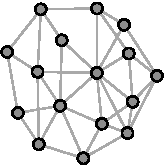
\includegraphics[width=.33\textwidth]{homophNet} & \hspace{2cm} &
  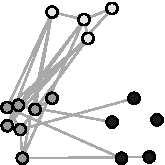
\includegraphics[width=.33\textwidth]{stochEquivNet}  
  \end{tabular}

}
%%%%%%%%%%%%%%%%%%%%%%%%%%%%%%%%%%%%%%%%%%%%%%%%%%%%%%%%%%%%

%%%%%%%%%%%%%%%%%%%%%%%%%%%%%%%%%%%%%%%%%%%%%%%%%%%%%%%%%%%%
\frame{
  \frametitle{Latent Variable Models}

  \begin{align}
  \begin{aligned}
  \text{Latent class model} \\
    &\alpha(u_{i}, u_{j}) = m_{u_{i}, u_{j}} \\
    &u_{i} \in \{1, \ldots, K \}, \; i \in \{1,\ldots, n\} \\
    &M \text{ a } K \times K \text{ symmetric matrix} \\
  \text{Latent distance model} \\
    &\alpha(\textbf{u}_{i}, \textbf{u}_{j}) = -|\textbf{u}_{i} - \textbf{u}_{j}| \\
    &\textbf{u}_{i} \in \mathbb{R}^{K}, \; i \in \{1, \ldots, n \} \\
  \text{Latent factor model} \\
    &\alpha(\textbf{u}_{i}, \textbf{u}_{j}) = \textbf{u}_{i}^{T} \Lambda \textbf{u}_{j} \\
    &\textbf{u}_{i} \in \mathbb{R}^{K}, \; i \in \{1, \ldots, n \} \\
    &\Lambda \text{ a } K \times K \text{ diagonal matrix}
  % \label{eqn:latAlpha}
  \end{aligned}
  \end{align}

}
%%%%%%%%%%%%%%%%%%%%%%%%%%%%%%%%%%%%%%%%%%%%%%%%%%%%%%%%%%%%

%%%%%%%%%%%%%%%%%%%%%%%%%%%%%%%%%%%%%%%%%%%%%%%%%%%%%%%%%%%%
\frame{
  \frametitle{Putting it together: AME}

\begin{align}
\begin{aligned}
  y_{ij} &= g(\theta_{ij}) \\ 
  &\theta_{ij} = \bm\beta^{T} \mathbf{X}_{ij} + e_{ij} \\
  &e_{ij} = a_{i} + b_{j}  + \epsilon_{ij} + \alpha(\textbf{u}_{i}, \textbf{v}_{j}) \text{  , where } \\
  &\qquad \alpha(\textbf{u}_{i}, \textbf{v}_{j}) = \textbf{u}_{i}^{T} \textbf{D} \textbf{v}_{j} = \sum_{k \in K} d_{k} u_{ik} v_{jk} \\ 
% \label{eqn:ame}
\end{aligned}
\end{align}

}
%%%%%%%%%%%%%%%%%%%%%%%%%%%%%%%%%%%%%%%%%%%%%%%%%%%%%%%%%%%%

%%%%%%%%%%%%%%%%%%%%%%%%%%%%%%%%%%%%%%%%%%%%%%%%%%%%%%%%%%%%
\frame{
  \frametitle{Swiss Climate Change Application}

\begin{figure}[ht]
  \centering
  \begin{tabular}{cc}
  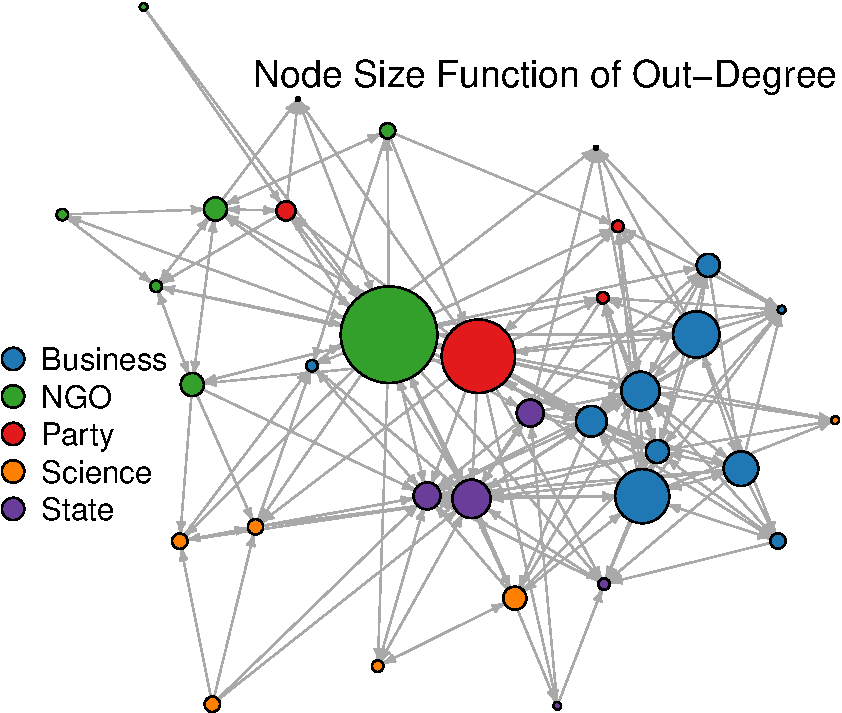
\includegraphics[width=.47\textwidth]{dvNet_outDegree} & 
  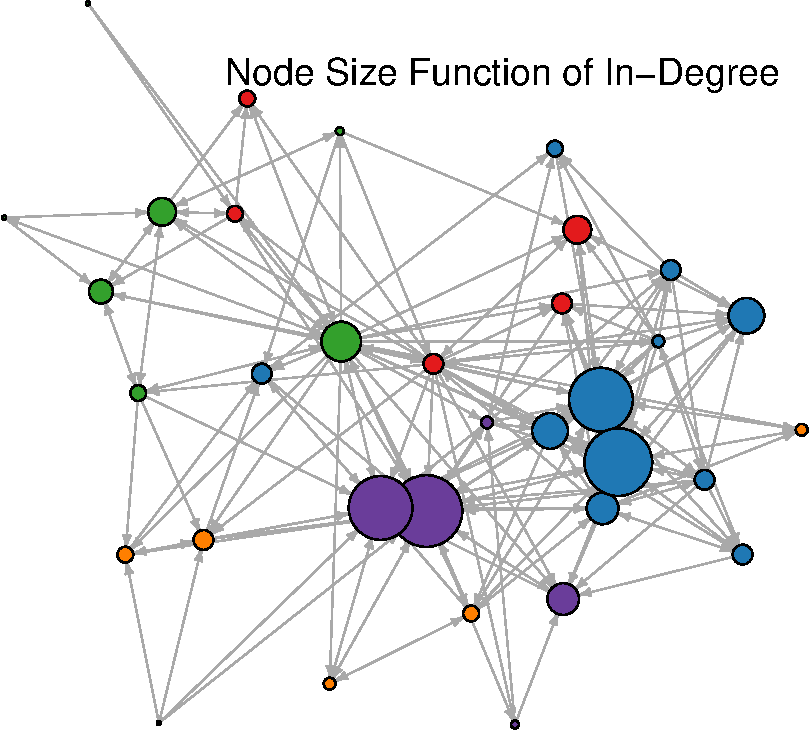
\includegraphics[width=.44\textwidth]{dvNet_inDegree}
  \end{tabular}
  % \caption{Network visualizations of the Swiss climate change mitigation network. Nodes are colored by type of actor, and directed edges indicate relationships between actors. The network on the left weights node size by the number of out-going ties, and on the right the number of incoming-ties.}
  % \label{fig:dvNet}
\end{figure}

}
%%%%%%%%%%%%%%%%%%%%%%%%%%%%%%%%%%%%%%%%%%%%%%%%%%%%%%%%%%%%

%%%%%%%%%%%%%%%%%%%%%%%%%%%%%%%%%%%%%%%%%%%%%%%%%%%%%%%%%%%%
\frame{
  \frametitle{Parameter Estimates}

\newcolumntype{L}{>{\arraybackslash}m{9cm}}
\begin{table}[ht]
\centering
\begingroup\scriptsize
\tiny{
\begin{tabular}{lcccccc}
\footnotesize{\textbf{Variable}} &  \footnotesize{\textbf{Expected}} & \footnotesize{\textbf{Logit}} & \footnotesize{\textbf{MRQAP}} & \footnotesize{\textbf{LSM}} & \footnotesize{\textbf{ERGM}} & \footnotesize{\textbf{AME}} \\ \hline\hline
  \multicolumn{2}{l}{\textbf{Conflicting policy preferences}} \\ 
  \quad Business v. NGO & $-$ & $-$ & $-$ & $+$ & $-$ & $-$ \\
  \quad Opposition/alliance  & $+$ & $-$ & $-$ & $+$ & $-$ & $-$ \\
  \quad Preference dissimilarity  & $-$ & $-$ & $-$ & $+$ & $-$ & $-$ \\
  \multicolumn{2}{l}{\textbf{Transaction costs}} \\ 
  \quad Joint forum participation  & $+$ & $-$ & $-$ & $+$ & $-$ & $-$ \\
  \multicolumn{2}{l}{\textbf{Influence}} \\ 
  \quad Influence attribution & $+$ & $-$ & $-$ & $+$ & $-$ & $-$ \\
  \quad Alter's influence in-degree  & $+$ & $-$ & $-$ & $+$ & $-$ & $-$ \\
  \quad Influence absolute diff.  & $-$ & $-$ & $-$ & $+$ & $-$ & $-$ \\
  \quad Alter = Government Actor & $+$ & $-$ & $-$ & $+$ & $-$ & $-$ \\
  \multicolumn{2}{l}{\textbf{Functional requirements}} \\ 
  \quad Ego = Environment NGO & $+$ & $-$ & $-$ & $+$ & $-$ & $-$ \\
  \quad Same actor type & $+$ & $-$ & $-$ & $+$ & $-$ & $-$ \\
  \multicolumn{2}{l}{\textbf{Endogenous dependencies: ERGM Specific Parameters}} \\ 
  \quad Outdegree popularity & $+$ & $-$ & $-$ & $+$ & $-$ & $-$ \\
  \quad Twopaths & $-$ & $-$ & $-$ & $+$ & $-$ & $-$ \\
  \quad GWIdegree (2.0) & $+$ & $-$ & $-$ & $+$ & $-$ & $-$ \\
  \quad GWESP (1.0) & $+$ & $-$ & $-$ & $+$ & $-$ & $-$ \\
  \quad GWOdegree (0.5) & $+$ & $-$ & $-$ & $+$ & $-$ & $-$ \\
\hline\hline
\end{tabular}
}
\endgroup
% \caption{Summary of variables to be included in model specification. With the exception of mutuality, each of the parameters falling in the Endogenous dependencies grouping are only explicitly testable through ERGM. }
% \label{tab:theorySpec}
\end{table}

}
%%%%%%%%%%%%%%%%%%%%%%%%%%%%%%%%%%%%%%%%%%%%%%%%%%%%%%%%%%%%

%%%%%%%%%%%%%%%%%%%%%%%%%%%%%%%%%%%%%%%%%%%%%%%%%%%%%%%%%%%%
\frame{
  \frametitle{Latent Factor Visualization}

  \centering
  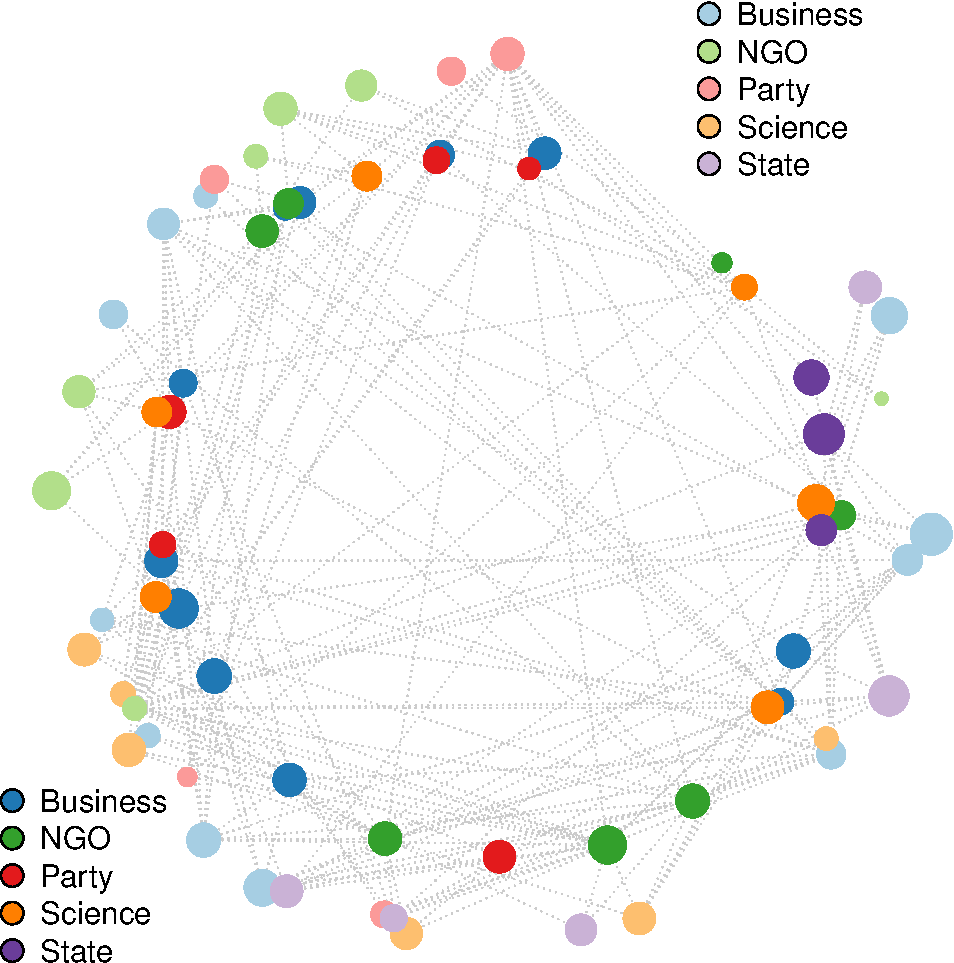
\includegraphics[width=.5\textwidth]{ameFitSR_2_UV}

}
%%%%%%%%%%%%%%%%%%%%%%%%%%%%%%%%%%%%%%%%%%%%%%%%%%%%%%%%%%%%

%%%%%%%%%%%%%%%%%%%%%%%%%%%%%%%%%%%%%%%%%%%%%%%%%%%%%%%%%%%%
\frame{
  \frametitle{Out of Sample Performance Assessment}

\begin{itemize}
  \item Randomly divide the $n \times (n-1)$ data points into $S$ sets of roughly equal size, letting $s_{ij}$ be the set to which pair $\{ij\}$ is assigned.
  \item For each $s \in \{1, \ldots, S\}$:
  \begin{itemize}
    \item Obtain estimates of the model parameters conditional on $\{y_{ij} : s_{ij} \neq s\}$, the data on pairs not in set $s$.
    \item For pairs $\{kl\}$ in set $s$, let $\hat y_{kl} = E[y_{kl} | \{y_{ij} : s_{ij} \neq s\}]$, the predicted value of $y_{kl}$ obtained using data not in set $s$.
  \end{itemize}
\end{itemize}

}
%%%%%%%%%%%%%%%%%%%%%%%%%%%%%%%%%%%%%%%%%%%%%%%%%%%%%%%%%%%%

%%%%%%%%%%%%%%%%%%%%%%%%%%%%%%%%%%%%%%%%%%%%%%%%%%%%%%%%%%%%
\frame{
  \frametitle{Performance Comparison}

\begin{tabular}{cc}
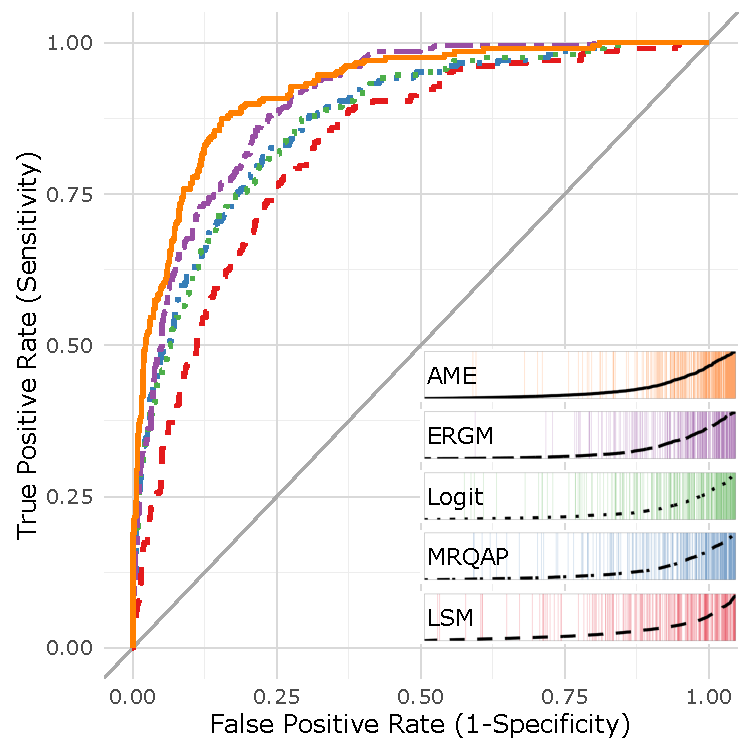
\includegraphics[width=.5\textwidth]{roc_outSample} & 
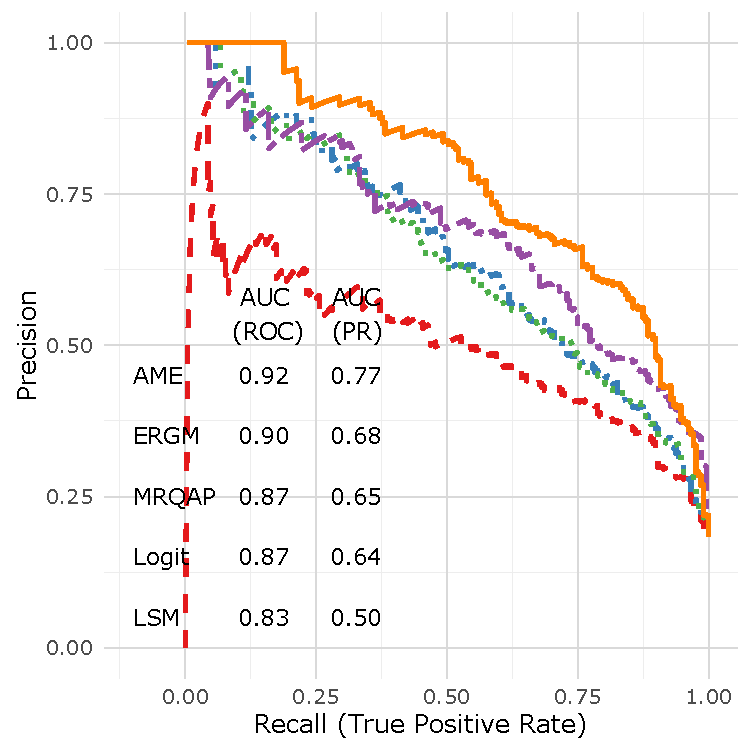
\includegraphics[width=.5\textwidth]{rocPr_outSample} 
\end{tabular}

}
%%%%%%%%%%%%%%%%%%%%%%%%%%%%%%%%%%%%%%%%%%%%%%%%%%%%%%%%%%%%

\frame{
  \frametitle{Network Dependencies}

  \centering
  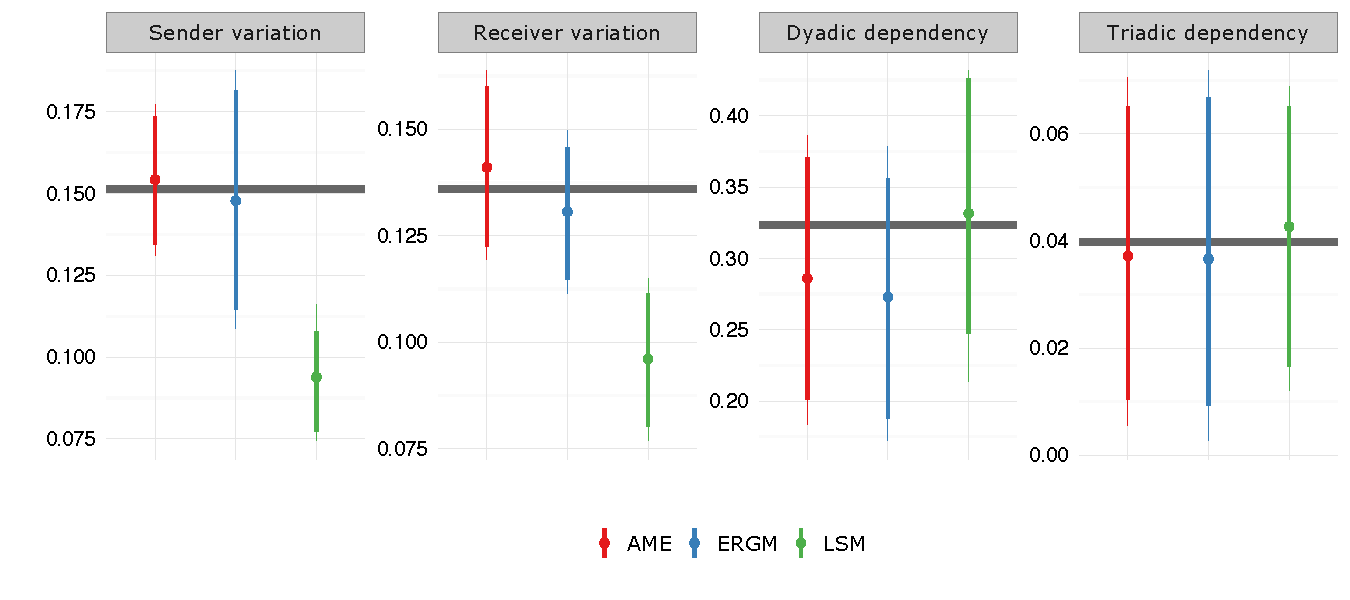
\includegraphics[width=1\textwidth]{netPerfCoef}

}

%%%%%%%%%%%%%%%%%%%%%%%%%%%%%%%%%%%%%%%%%%%%%%%%%%%%%%%%%%%%
\plain{Thanks.}
%%%%%%%%%%%%%%%%%%%%%%%%%%%%%%%%%%%%%%%%%%%%%%%%%%%%%%%%%%%%

%%%%%%%%%%%%%%%%%%%%%%%%%%%%%%%%%%%%%%%%%%%%%%%%%%%%%%%%%%%%
\frame{
  \frametitle{Standard Network Dependence Measures}
\vspace{-5mm}
\includegraphics[width=1\textwidth]{ggGofAll_preeze}
}
%%%%%%%%%%%%%%%%%%%%%%%%%%%%%%%%%%%%%%%%%%%%%%%%%%%%%%%%%%%%

%%%%%%%%%%%%%%%%%%%%%%%%%%%%%%%%%%%%%%%%%%%%%%%%%%%%%%%%%%%%
\frame{
  \frametitle{Simulation Comparison}

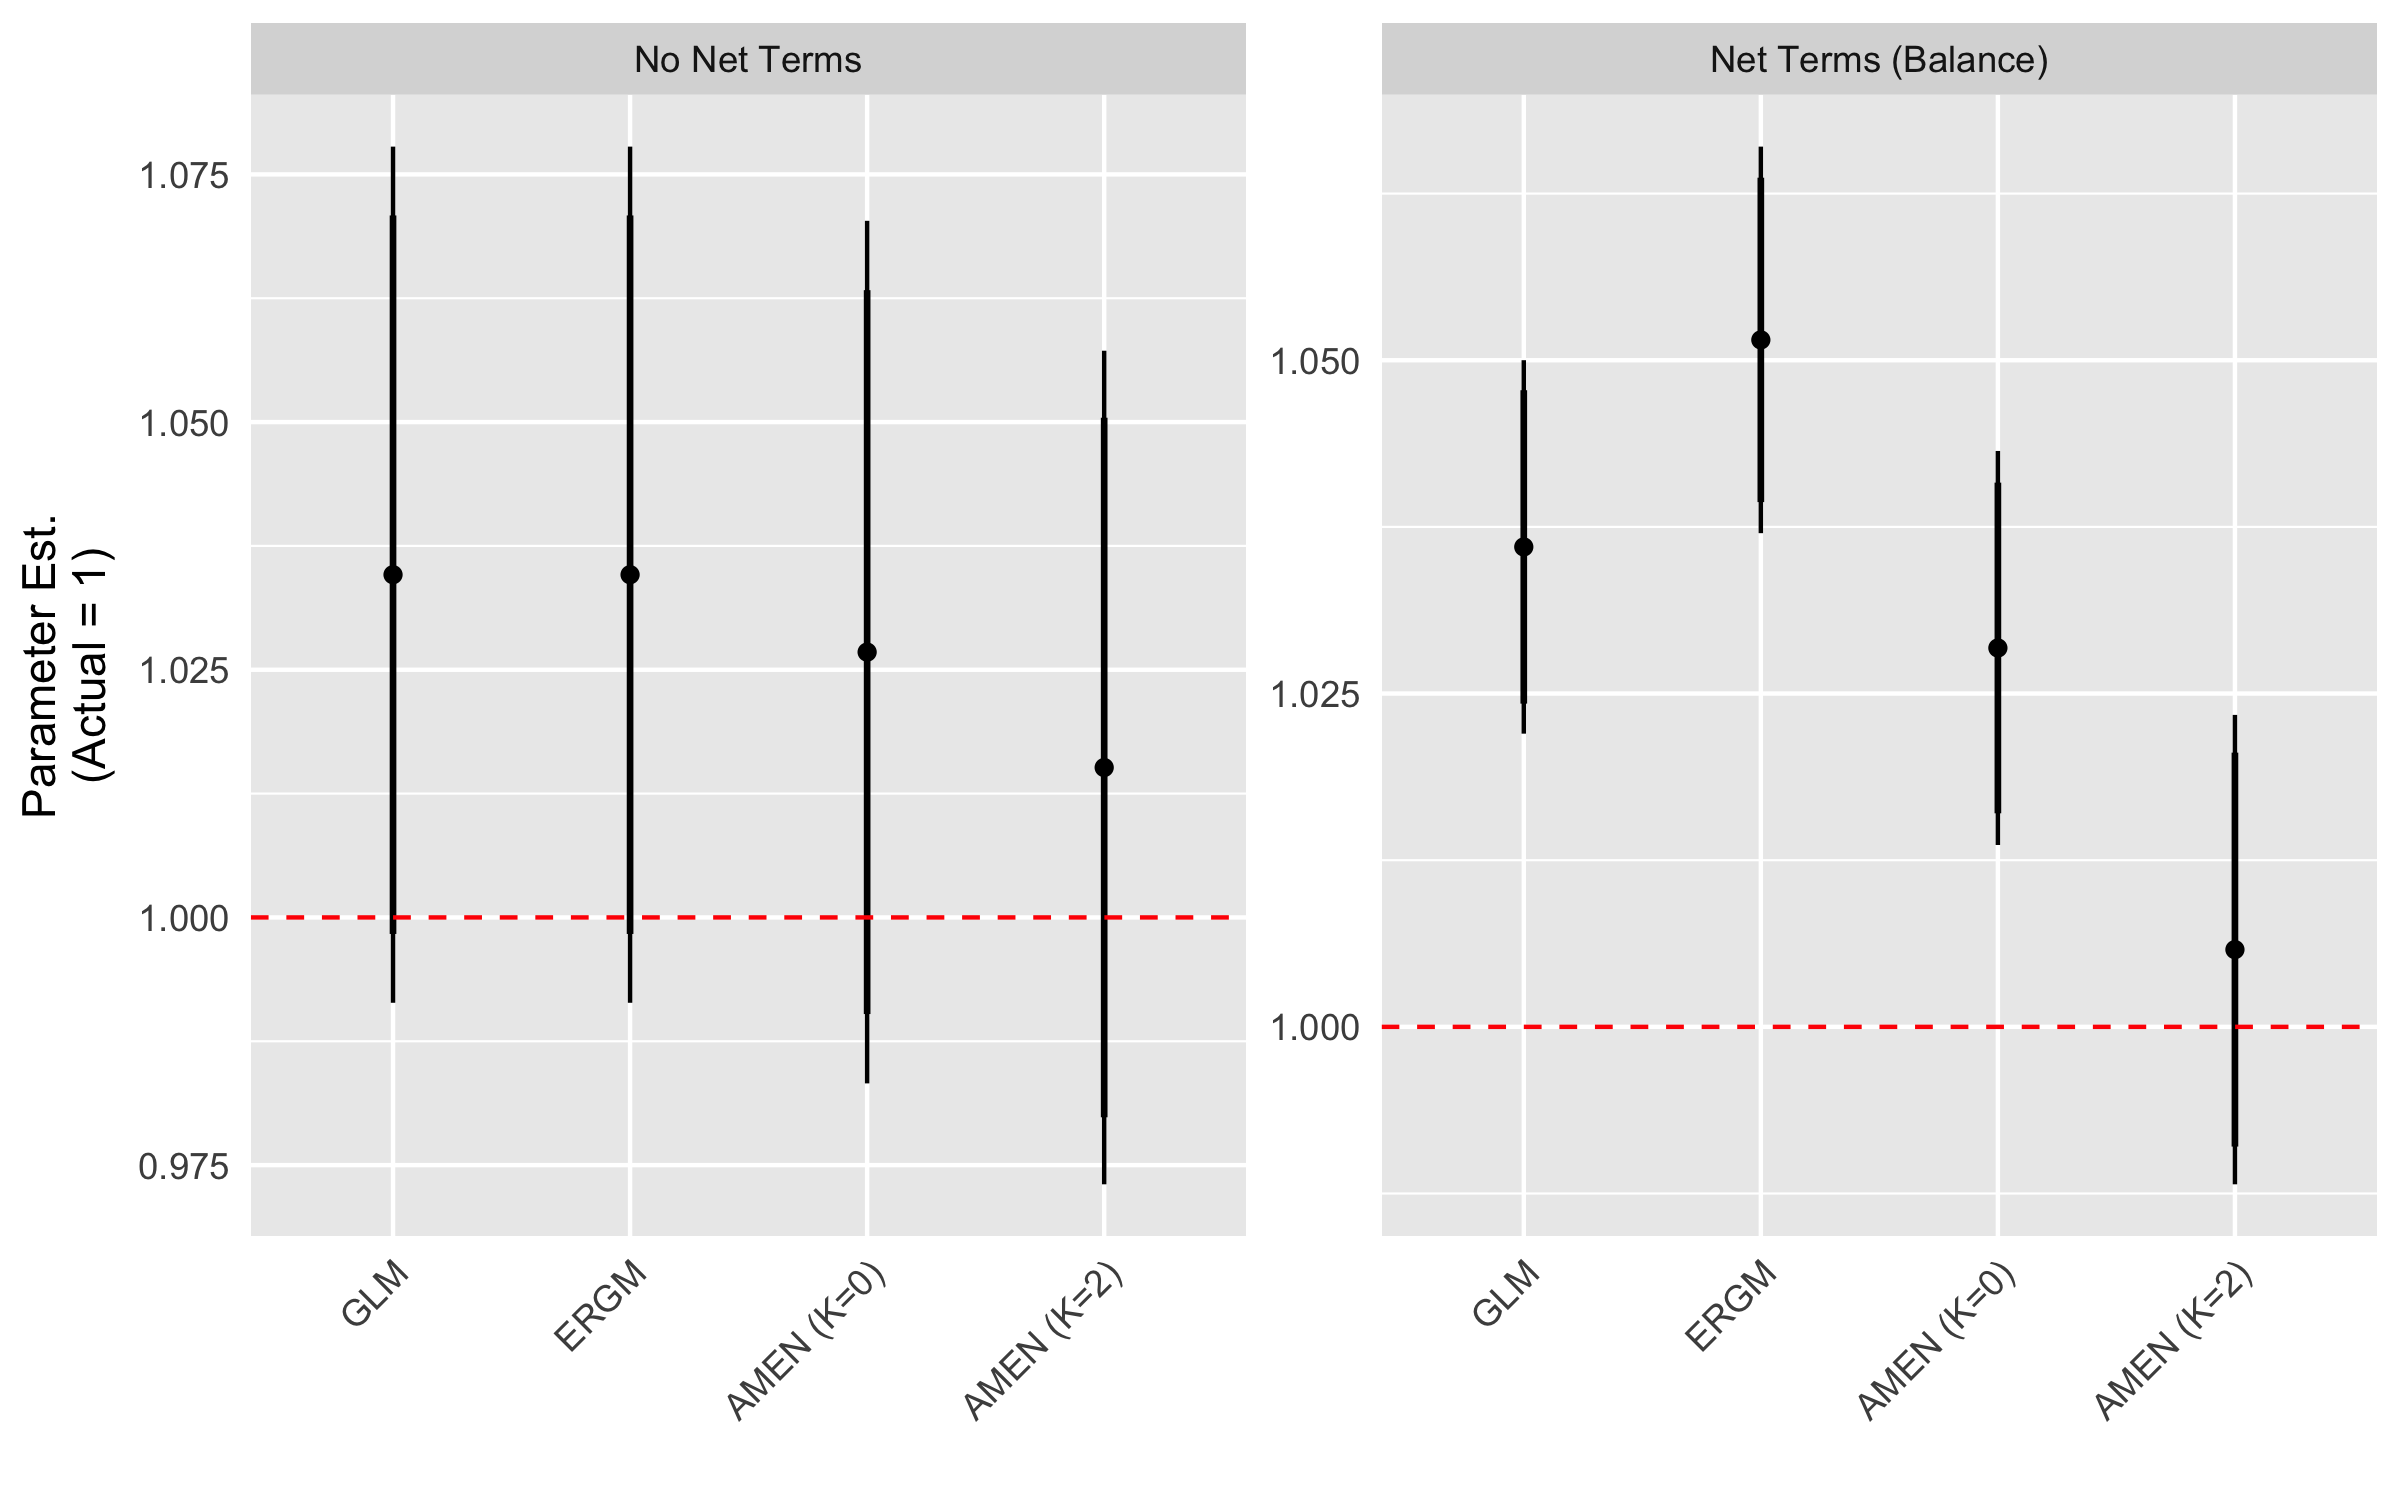
\includegraphics[width=1\textwidth]{ameVergmSim.png}

}
%%%%%%%%%%%%%%%%%%%%%%%%%%%%%%%%%%%%%%%%%%%%%%%%%%%%%%%%%%%%

%%%%%%%%%%%%%%%%%%%%%%%%%%%%%%%%%%%%%%%%%%%%%%%%%%%%%%%%%%%%
\frame{
  \frametitle{AMEN v LSM Performance}

  \begin{tabular}{cc}
  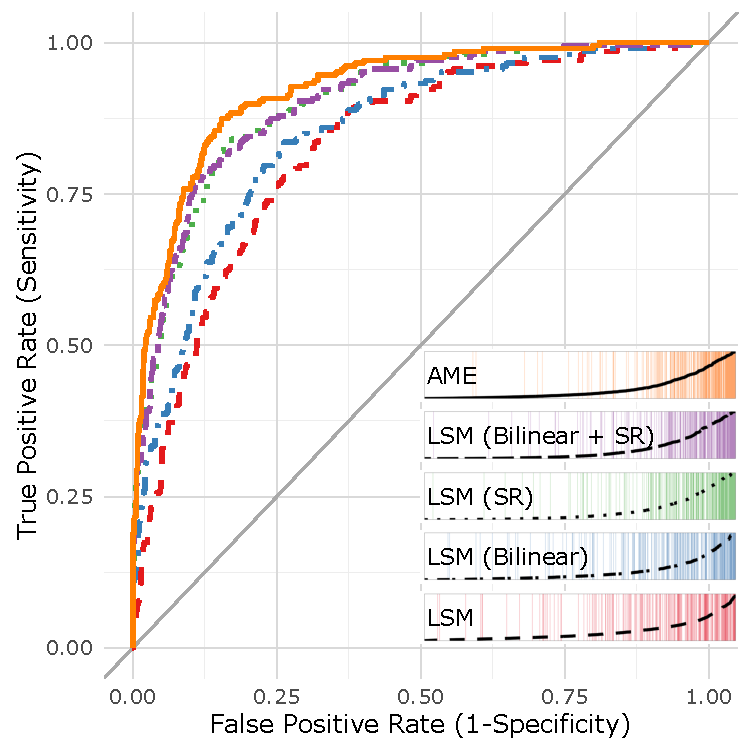
\includegraphics[width=.5\textwidth]{roc_latSpace_outSample} & 
  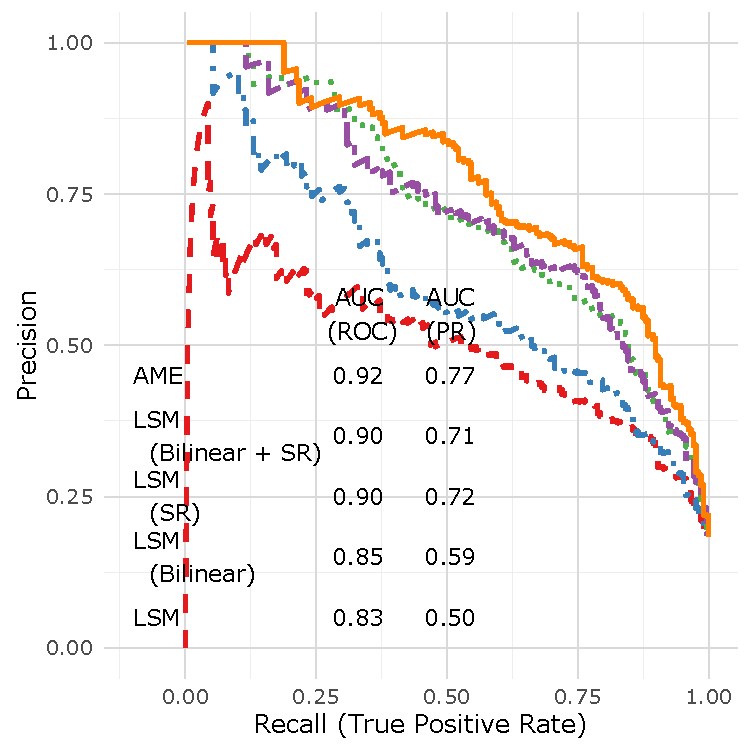
\includegraphics[width=.5\textwidth]{rocPr_latSpace_outSample}
  \end{tabular}

}
%%%%%%%%%%%%%%%%%%%%%%%%%%%%%%%%%%%%%%%%%%%%%%%%%%%%%%%%%%%%

%%%%%%%%%%%%%%%%%%%%%%%%%%%%%%%%%%%%%%%%%%%%%%%%%%%%%%%%%%%%
\frame{
  \frametitle{AMEN V LSM Net Dependence}

  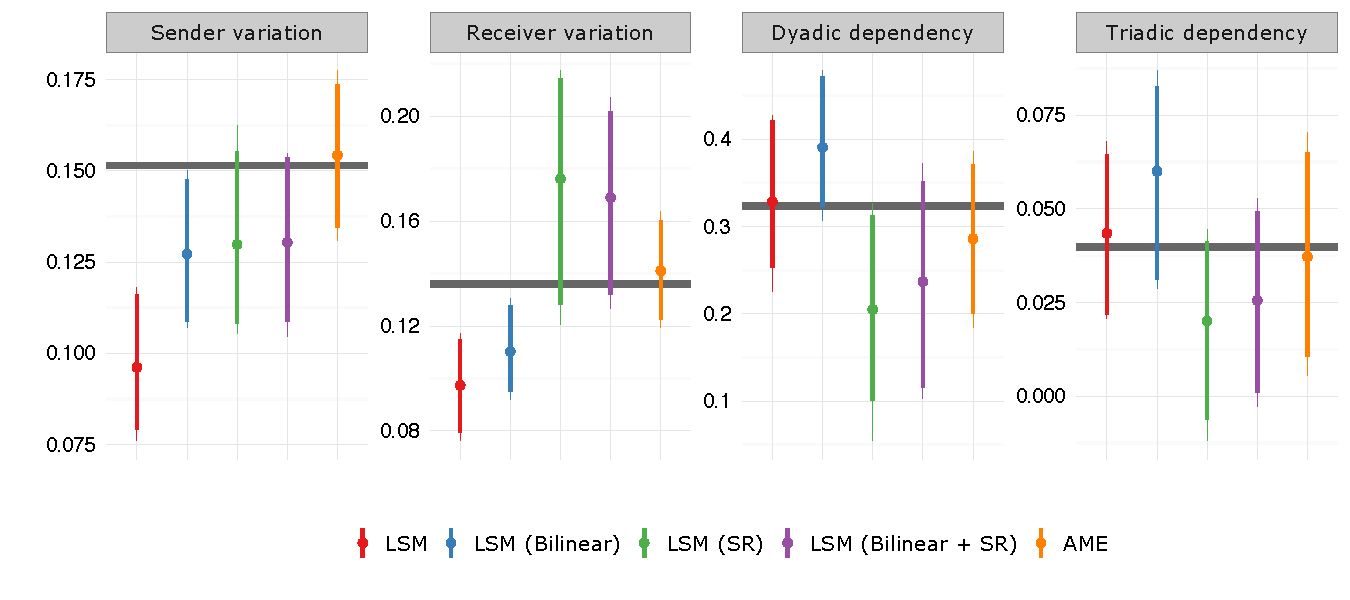
\includegraphics[width=1\textwidth]{netPerfCoef_latSpace}
}
%%%%%%%%%%%%%%%%%%%%%%%%%%%%%%%%%%%%%%%%%%%%%%%%%%%%%%%%%%%%

%%%%%%%%%%%%%%%%%%%%%%%%%%%%%%%%%%%%%%%%%%%%%%%%%%%%%%%%%%%%
\frame{
  \frametitle{AMEN v LSM Performance}

  \begin{tabular}{cc}
  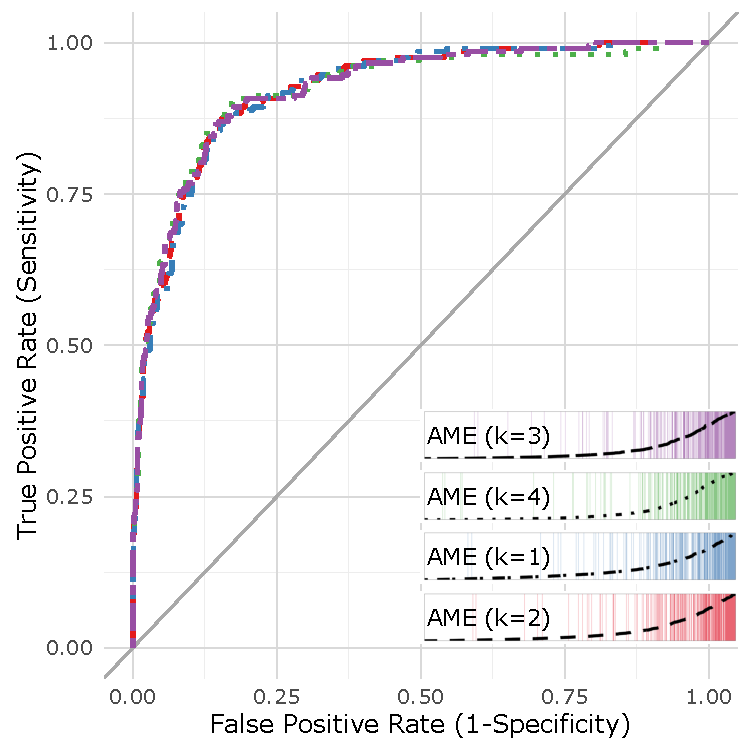
\includegraphics[width=.5\textwidth]{roc_ameSR_outSample} & 
  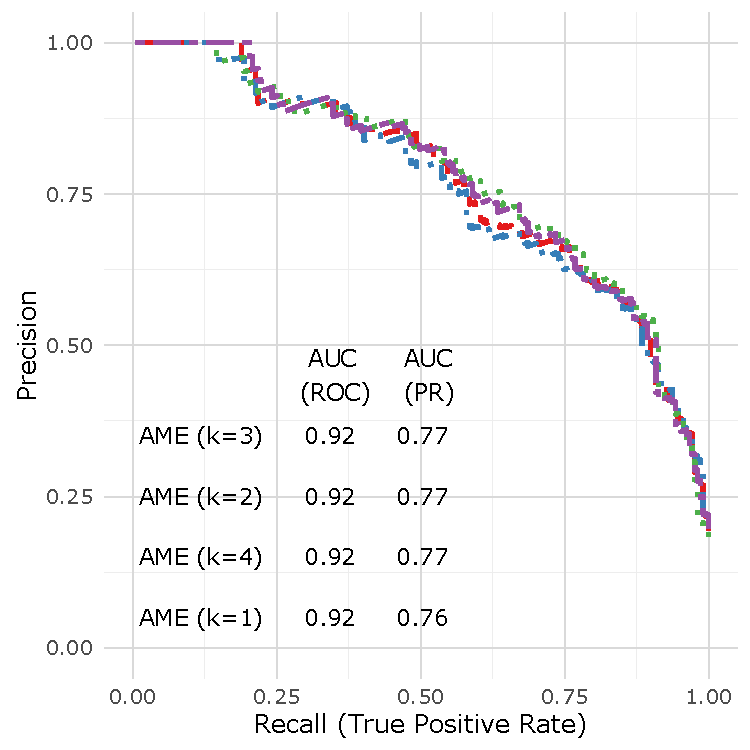
\includegraphics[width=.5\textwidth]{rocPr_ameSR_outSample}
  \end{tabular}

}
%%%%%%%%%%%%%%%%%%%%%%%%%%%%%%%%%%%%%%%%%%%%%%%%%%%%%%%%%%%%

%%%%%%%%%%%%%%%%%%%%%%%%%%%%%%%%%%%%%%%%%%%%%%%%%%%%%%%%%%%%
\frame{
  \frametitle{AMEN V LSM Net Dependence}

  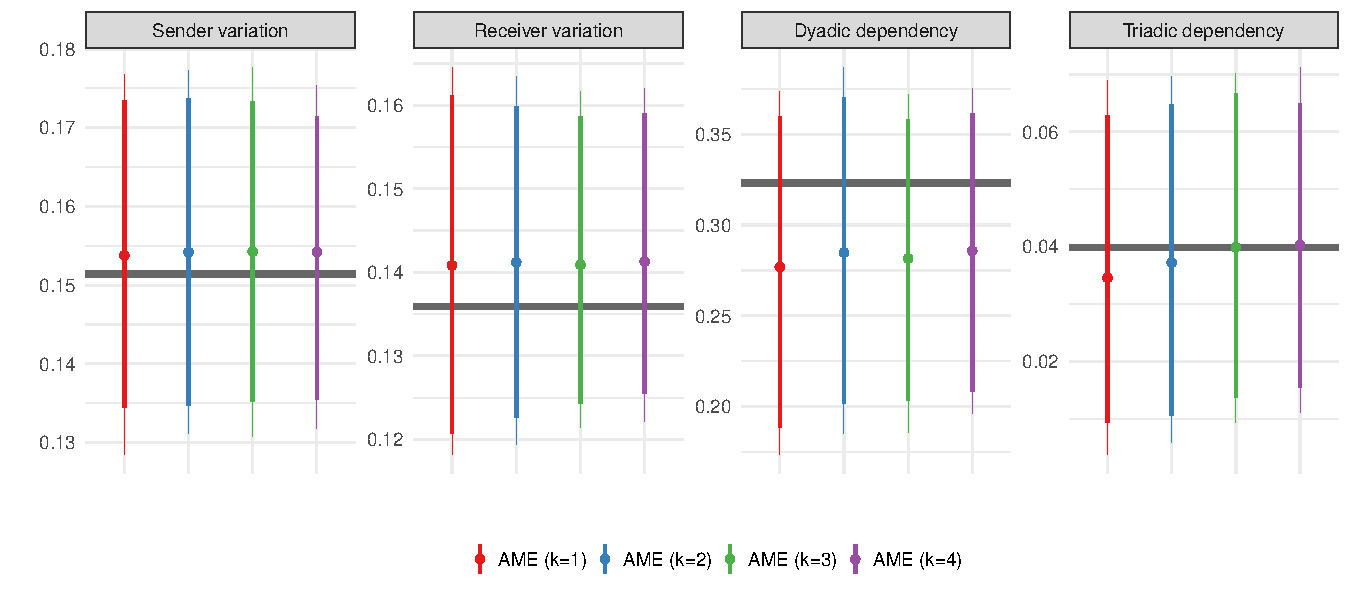
\includegraphics[width=1\textwidth]{netPerfCoef_ameSR}
}
%%%%%%%%%%%%%%%%%%%%%%%%%%%%%%%%%%%%%%%%%%%%%%%%%%%%%%%%%%%%

\end{document}
